\documentclass[tikz,border=2]{standalone}
\usetikzlibrary{shadows,arrows,shapes,positioning,calc,backgrounds,fit}
\newcommand{\vanish}[1]{}
\usepackage{colortbl}
\usepackage{array}
\usepackage{amssymb}
\usepackage{multirow}
\newcommand{\shaded}[1]{\cellcolor{black!20}{#1}}
\newcommand{\calc}[1]{\mbox{$\mathcal{C}_{#1}$}}
\pdfpageattr {/Group << /S /Transparency /I true /CS /DeviceRGB>>}
\newcommand{\mathtttt}{}
% Define the layers to draw the diagram
%
\begin{document}
%% \pgfdeclarelayer{bg}
%% \pgfdeclarelayer{fg}
%% \pgfsetlayers{bg,main,fg}
%
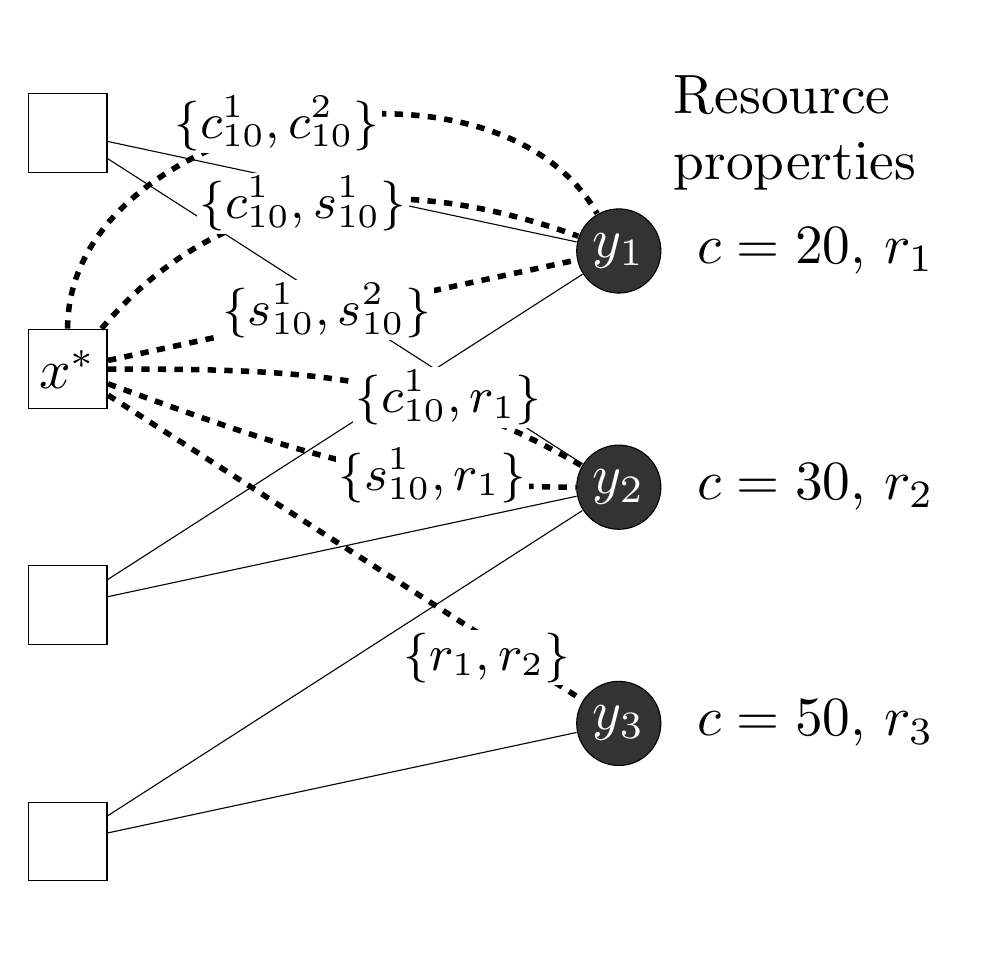
\begin{tikzpicture}
[scale=2,node distance=.5cm, transform shape,
    agent/.style={draw,minimum
    width=.5cm,minimum height=.5cm,text=black,shape=rectangle,inner sep=.5mm},
    res/.style={shape=circle,fill=black!80,text=white,draw,inner sep=.5mm},
    lab/.style={fill=white,font=\small,inner sep=.5pt},
    prop/.style={text width=2cm},
myedge/.style={>=latex', shorten >=.0pt, shorten <=.0pt,semithick},
inc/.style={dashed,line width=2pt}]
%%%%%%%%%%
%% \begin{scope}
%%     \node[text width=9cm] (desc) {
%% Agent set~$\{x_1,x_2,x_3,x_4\}$; Resource set~$\{y_1,y_2,y_3\}$\\ 
%% Attributes: class seating capacity~$c$ and location~$r_j$\\
%% Agent seeking advice is~$x^*=x_2$ with the following preferences:
%% $c\ge 30$ and $r_2>r_1>r_3$. It also has the option of increasing the
%% seating capacity ($s_{10}$) for a fee.};
%% \end{scope}
%%
%% \draw (desc.south west) -- (desc.south east);
\begin{scope}[shift={(-2.5,-2)}]
%% nodes
\node (x1) [agent] at (0,0)  {};
\node (x2) [agent] at (0,-1.5) {$x^*$};
\node (x3) [agent] at (0,-3) {};
\node (x4) [agent] at (0,-4.5) {};
\node (y1) [res] at (3.5,-.75) {$y_1$};
\node (y2) [res] at (3.5,-2.25) {$y_2$};
\node (y3) [res] at (3.5,-3.75) {$y_3$};
%% resource properties
\node (py1) [right=of y1,shift={(-.4,0)}] {$c=20$, $r_1$};
\node (py2) [right=of y2,shift={(-.4,0)}] {$c=30$, $r_2$};
\node (py3) [right=of y3,shift={(-.4,0)}] {$c=50$, $r_3$};
\node (trp) [text width=1.8cm] at (py1|-x1) {Resource \\properties};
%% edges
\draw (x1) -- (y1); 
\draw (x1) -- (y2); 
\draw (x3) -- (y1); 
\draw (x3) -- (y2); 
\draw (x4) -- (y2); 
\draw (x4) -- (y3); 
%%
\draw[inc,out=90,in=120] (x2) edge node[lab,shift={(-.1,0)}]{$\{
\mathtttt{c^1_{10}},\mathtttt{c^2_{10}}\}$} (y1); 
\draw[inc,out=50,in=160] (x2) edge node[lab,shift={(-.1,0)}]{$\{
\mathtttt{c^1_{10}},\mathtttt{s^1_{10}}\}$} (y1); 
\draw[inc] (x2) edge node[lab,shift={(-.1,0)}]{$\{
\mathtttt{s^1_{10}},\mathtttt{s^2_{10}}\}$} (y1); 
\draw[inc,out=0,in=150] (x2) edge
node[lab,shift={(.6,-.1)}]{$\{\mathtttt{c^1_{10}},r_1\}$} (y2); 
\draw[inc,out=-20,in=180] (x2) edge
node[lab,shift={(.6,-.1)}]{$\{\mathtttt{s^1_{10}},r_1\}$} (y2); 
\draw[inc] (x2) edge node[lab,shift={(.9,-.7)}]{$\{\mathtttt{r_1},
\mathtttt{r_2}\}$} (y3); 
%%
\node (anc) at ($(x4.south)+(0,-.2)$) {};
%%\node [inner sep=3mm,draw,circle] at (x2) {};
\end{scope}
%%
%% \node[text width=9cm] at (0,-8) (incset) {Here, the incompatibility
%% set~$\Gamma$ consists of the following resource--restrictions pair:
%% $(y_1,\{c_{30},r_2\})$, $(y_1,\{s_{10},r_2\})$,
%% $(y_2,\{c_{30}\})$, $(y_2,\{s_{10}\})$, and $(y_3,\{r_2,r_1\})$.};
%% \draw (incset.north west) -- (incset.north east);
\end{tikzpicture}
\end{document}
